\chapter{Avaliação dos Extratores de Tópicos}\label{cap-extratores}

% Dar uma geral nesse primeiro parágrafo
	% Escolha dos Algorítmos
	% Escolha do método de avaliação (subjetivo com questionario)

% -- 1 - Motivação para o experimento.
Nesse capítulo, as técnicas de extração de tópicos são analisadas. O objetivo é comparar os algoritmos de extração de tópicos na tarefa de extração de padrões no contexto das atas de reunião no que tange a qualidade dos agrupamentos e seus descritores bem como sua capacidade de representar os segmentos. Escolheu-se os modelos LDA, PLSA e K-Means para essa análise devido a popularidade desses métodos os quais são amplamente utilizados~\cite{DZhu20122} e frequentemente referenciados em trabalhos voltados a organização de bases textuais~\cite{Aggarwal2018, OCallaghan2015, Steyvers2007}.
Os algoritmos foram inicialmente configurados com base em avaliações internas~\cite{Hassani2017} e observações empíricas nas quais escolheu-se os melhores valores para seus parâmetros. Os resultados desses modelos foram submetidos a uma avaliação subjetiva a fim de analisá-los junto a usuários com afinidade com atas de reuniões. 

Nessa avaliação, a técnica de segmentação textual também foi avaliada, uma vez que é a etapa anterior a extração de tópicos está diretamente ligada a os resultados apresentados ao avaliador bem como pode interferir no funcionamento dos modelos de extração de tópicos. Assim, a técnica de segmentação textual foi avaliada subjetivamente em complemento a análise estatística apresentada no Capítulo~\ref{cap-segmentadores}.

A avaliação se deu por meio de questionários onde profissionais com afinidade com atas de reunião forneceram suas percepções em relação aos resultados dos modelos de extração de tópicos. Por fim, os dados serviram como base para análise dos algoritmos 


\section{Configuração experimental}

% A qtd de tópicos é um parametro importante.
% Todos com 70 tópicos e 5 extratores;
Durante os primeiros testes empíricos a qualidade dos resultados mostrou-se sensível à quantidade de tópicos extraídos.
Inicialmente, realizou-se um teste prévio utilizando uma versão não-paramétrica dos algorítimos a fim de automaticamente obter valores ótimos para esse parâmetro por meio da análise das medidas Silhueta e Coesão. Essa configuração automática resulta valores em torno de 20 tópicos. Contudo, apresenta grupos com muitos segmentos (em torno de 100) o que os tornam pouco coesos além de certa dificuldade em julgar capacidade dos descritores em representar bem o tópico.  
Em observações diretas, valores próximos a entre 60 e 80 mostraram melhores resultados. Nesse trabalho, optou-se por configurar os extratores para extrair 70 tópicos da coleção de segmentos por apresentar melhor resultados aparente na visão de usuário.

Outro fator importante é a quantidade de descritores selecionados para cada tópico. Com base no experimento de anotações em segmentação, descrito no Capítulo~\ref{cap2}, os anotadores selecionaram em média 5 palavras para descrever os segmentos, sendo esse valor adotado para essa avaliação.




\section{Critérios de avaliação}


% - Explicar que foram 2 consultas (quais) e mostrar os extratores.
% - 4 - Procedimento (2 consultas, técnicas em ordens diferentes).
Após a configuração, cada um dos modelos de extração de tópicos foi submetido a duas consultas: ``\textit{compra de equipamentos}'' e ``\textit{defesa de dissertação}'' gerando 6 cenários distintos a serem analisados. 
Para cada cenário, o sistema seleciona o tópico com maior relevância com a consulta e em seguida exibe 5 segmentos desse tópico escolhidos aleatoriamente. 
Vale dizer que nessa avaliação as técnicas de ranqueamento dos resultados não são aplicadas para que estas não interfiram na avaliação dos extratores, contudo, o sistema final poderá ranquear também os segmentos com maior relevância de um ou mais tópicos por meio de técnicas de recuperação de informação. 
Os resultados desses cenários foram apresentados a um grupo de avaliadores que individualmente avaliaram a qualidade das técnicas de extração de tópicos. 
%

% -- 3 - Escolha dos participantes.
O perfil dos avaliadores é de profissionais da area acadêmica/escolar devido à sua afinidade com o ambiente de gestão e conhecimentos de assuntos relacionados ao \textit{corpus} estudado nesse trabalho. O grupo convidado a participar do experimento é formado por 24 profissionais da UFSCar campus Sorocaba, 13 profissionais de escolas técnicas e 3 profissionais de escolas do Ensino Fundamental, sendo 11 ocupantes de cargos de gestão como coordenadores de curso, diretores, 17 membros de conselhos, 5 profissionais administrativos e 3 professores, totalizando 40 avaliadores em que a maioria afirma ter afinidade com atas e reuniões e 3 declararam nenhuma afinidade com esses documentos. Os avaliadores foram divididos em dois grupos onde cada grupo avaliou as técnicas de extração tópicos a partir de uma consulta (palavras-chave), ou seja, cada indivíduo avaliou 3 cenários distintos. A avaliação consistiu de um documento impresso contendo uma breve apresentação do trabalho, seguido de uma cópia dos resultados das técnicas de extração de tópicos e questões avaliativas sobre cada técnica.

% X profissionais de gestão de instituições 

% -- 2 - Escolha das questões.
O questionário foi formado por questões envolvendo aspectos os extratores de tópicos e questões referentes à técnica de segmentação textual empregada
As respostas seguiram a escala \textit{Likert}~\cite{Norman2010} com 5 alternativas. 
% , conforme mostrado:

\begin{enumerate}
	\item Todos os trechos apresentados compartilham um mesmo assunto.
	\item As palavas \textit{<descritores>} resumem bem o assunto tratado nos trechos.
	\item Existem trechos que não tratam de um único assunto?
	\item Existem trechos incompletos e insuficientes para compreensão do assunto do trecho?
\end{enumerate}


As questões 1 e 2 estão relacionadas ao extrator de tópicos. A primeira refere-se ao agrupamento dos segmentos pela qual foi avaliada a semelhança dos trechos em termos de assunto. A segunda questão diz respeito aos descritores selecionados, ao respondê-la o avaliador indicou o quão bem esses termos representam aquele grupo.
As questões 3 e 4 estão ligadas à técnica de segmentação utilizada, o BayesSeg conforme já mencionado no Capítulo~\ref{cap-segmentadores}. A questão 3 está ligada à coesão de cada segmento, levando em conta a homogeneidade do texto em relação a um assunto. A questão 4 refere-se a completude dos segmentos, ou seja, o quão bem os segmentos podem ser bem compreendidos independentemente da leitura do documento integral.


% -- 5 - Escolha dos temas para consulta: 






% Nesse trabalho, os algoritmos de extração de tópicos foram avaliados subjetivamente. 

\section{Resultados}


Os dados coletados das avaliações foram analisados



\begin{figure}[!h] \centering     %%% not \center

	\subfigure{ \label{fig:kmeans}
		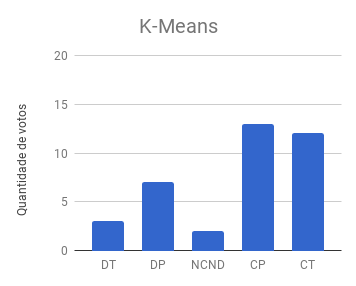
\includegraphics[width=.31\textwidth]{conteudo/capitulos/figs/figuras-experimento/Q1-KMeans.png}
	}	
	\subfigure{ \label{fig:lda}
		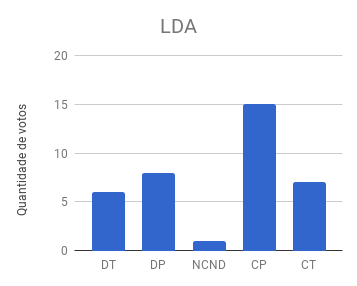
\includegraphics[width=.31\textwidth]{conteudo/capitulos/figs/figuras-experimento/Q1-LDA.png}
	}
	\subfigure{ \label{fig:plsa}
		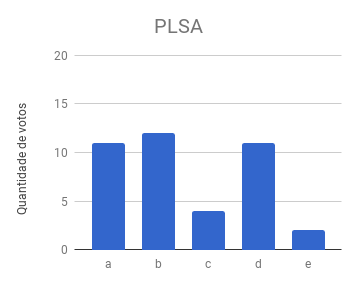
\includegraphics[width=.31\textwidth]{conteudo/capitulos/figs/figuras-experimento/Q1-PLSA.png}
	}
	\caption{ \textit{``Todos os trechos apresentados compartilham um mesmo assunto.''} }
	\label{fig:exemplomatrixrank}
\end{figure}




\begin{figure}[!h] \centering     %%% not \center

	\subfigure{ \label{fig:kmeans}
		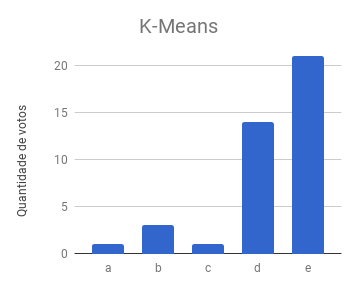
\includegraphics[width=.31\textwidth]{conteudo/capitulos/figs/figuras-experimento/Q2-KMeans.png}
	}	
	\subfigure{ \label{fig:lda}
		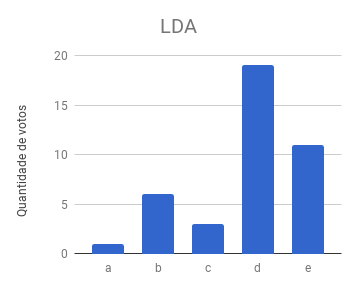
\includegraphics[width=.31\textwidth]{conteudo/capitulos/figs/figuras-experimento/Q2-LDA.png}
	}
	\subfigure{ \label{fig:plsa}
		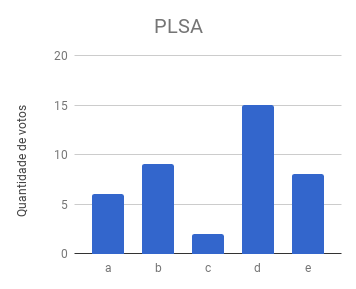
\includegraphics[width=.31\textwidth]{conteudo/capitulos/figs/figuras-experimento/Q2-PLSA.png}
	}
	\caption{\textit{``As palavas <descritores> resumem bem o assunto tratado nos trechos.''} }
	\label{fig:exemplomatrixrank}
\end{figure}





\begin{figure}[!h] \centering     %%% not \center

	\subfigure{ \label{fig:kmeans}
		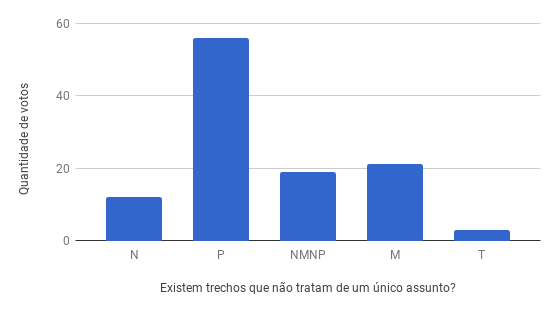
\includegraphics[width=.31\textwidth]{conteudo/capitulos/figs/figuras-experimento/Q3-Seg.png}
	}	
	\subfigure{ \label{fig:lda}
		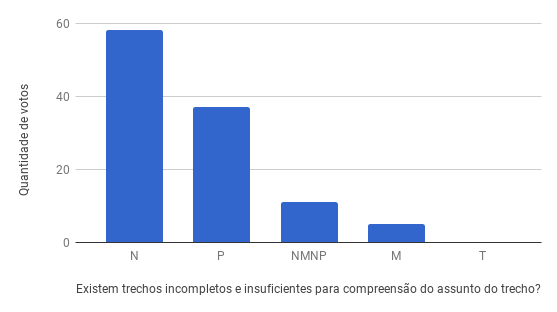
\includegraphics[width=.31\textwidth]{conteudo/capitulos/figs/figuras-experimento/Q4-Seg.png}
	}
	\caption{\textit{``Existem trechos que não tratam de um único assunto?''} \textit{``Existem trechos incompletos e insuficientes para compreensão do assunto do trecho?''} }
	\label{fig:exemplomatrixrank}
\end{figure}






